\documentclass{article}

\title{Impact of Network Topology on Cooperation in Public Goods Games}
\date{2018-11-11}
\author{John M. Maloney}

\usepackage{booktabs}
\usepackage{multirow}
\usepackage{amsmath}
\usepackage{tabu}
\usepackage{array}
\usepackage{graphicx}
\usepackage{subcaption}

\begin{document}

  \maketitle

  \section{Introduction}
  Both evolutionary processes as well as economic marketplaces are driven by competition between individuals. It would appear that only selfish behavior would be rewarded.  However, cooperation and altruistic behavior is witnessed throughout the natural world and in human societies.  Explaining the existence of these cooperative and altruistic behaviors is a challenge for both evolutionary biology and economics.  If the cooperators are closely related, altruistic cooperation can be seen as benefiting reproduction of the shared gene set.  However, cooperation also occurs among unrelated individuals and this reciprocity-based cooperation is harder to explain.
  \paragraph{}Lacking the ability to manipulate natural and economic systems in order to conduct experiments that could confirm or deny theories about the evolution of cooperation, scientists use mathematical modeling and simulation to test their hypotheses.  The game theoretic constructs known as the prisoner's dilemma game and the donor-recipient game are often used as the basis for these investigations.
  \paragraph{}In \cite{Maloney2015a}, the eight social norms used to promote cooperation in the donor-recipient game \cite{Ohtsuki2006} were applied to the public goods game.  Those results showed that none of the social norms is evolutionary stable.  In this study, experiments are conducted to analyze the impact that population structure has on the evolution of cooperation in public goods games.
  \paragraph{}The rest of this paper is structured as follows:  section 2 covers related work on the impact of network topology on the evolution of cooperation in the prisoner's dilemma, section 3 presents an extension of the models and methodologies presented in section 2 to the public goods game, section 4 presents the experimental results, section 5 concludes the paper and presents ideas for future work.
  
    \section{Population Structure in the Prisoner's Dilemma Game}
    This section provides an overview of related work that analyzes the impact of population structure on the evolution of cooperation in the repeated 2-person prisoner's dilemma game.  First, a brief description of the repeated 2-person prisoner's dilemma game is provided.  Next, studies that consider the case of a fixed network topology are reviewed.  Finally, studies that consider the case in which agents can modify the network topology are reviewed.
    
    \subsection{Prisoner's Dilemma Game}
    \paragraph{}In the two-player prisoner's dilemma game, each player can take one of two actions: cooperate or defect.  After each player chooses an action, the players receive the payouts shown in table \ref{table:pdpayouts}.
    
    \begin{table}[h]
      \begin{center}
      \begin{tabular}{llcc}
    	\toprule
		&	&	\multicolumn{2}{c}{Player 2} \\ \cmidrule{3-4}
		&   & 	Cooperate & Defect  \\ \midrule
    	\multirow{2}{*}{Player 1}
    		& Cooperate   & R  & S  \\
    		& Defect  	  & T  & P \\ \bottomrule
      \end{tabular}
      \caption{The Prisoners Dilemma Game}
      \label{table:pdpayouts}
	  \end{center}
    \end{table}

    \paragraph{}The payouts are constrained as follows in order to create a social dilemma:

    \begin{equation}
    	T > R > P > S
    \end{equation}
    
    \paragraph{}Given the order of the payouts, if the players only play the game once, regardless of the action chosen by the other player, the highest payout is always achieved by defecting.  Therefore, two rational players engaged in the game will both choose to defect and therefore receive the second lowest possible payout.  However, if both players choose to cooperate, they both receive a higher payout.  Thus, a social dilemma exists.
    \paragraph{}Rather than focusing on determining the optimal strategy to be played when two players meet in a single round of the game, evolutionary game theory considers which strategies will be most successful when the game is played during multiple interactions between agents following different strategies.  The fitness of a strategy is evaluated in terms of the payouts earned by agents that follow that strategy and is used to determine how many offspring in the next generation will follow that strategy.  In this case, evolutionary game theory tries to determine which strategies will be most evolutionarily successfully rather than which strategy is the most rational.

    \subsection{Impact of Network Topology on Evolution of Cooperation} \label{impact-net-topology}
    In this section, studies are reviewed that demonstrate the sensitivity of cooperation to the topology of the network occupied by the agents.  In the cases considered here, the network topology remains fixed during the simulation.  Although some of the studies reviewed consider the impact on cooperation in games other than the prisoner's dilemma, this review focuses on the results reported for the prisoner's dilemma.
    \paragraph{}All studies, except \cite{Santos2006c}, use the following payout structure that was originally used in \cite{Nowak1992}:

    \begin{align}
    	R&=1\\
    	T-b&>R\\
    	P&=S=0
    \end{align}

    \paragraph{}Given this structure for the payouts, b is the sole parameter and represents the temptation to defect.  In \cite{Santos2006c}, the authors broaden the range of payouts considered for the prisoner's dilemma game to include values for S between zero and -1.  However, in what follows only results presented in \cite{Santos2006c} for payouts that are compatible with the structure presented above as considered.
    \paragraph{}In each study, agents are allocated to the nodes of a graph with a fixed number of nodes equal to the number of agents n.  The graph has a fixed number of edges giving the graph a fixed average connectivity z.  The agents follow one of two strategies: unconditional cooperation or unconditional defection.
    \paragraph{}For each generation, each agent plays the social dilemma game being investigated with each of its neighbors achieving a fitness score equal to the sum of the payouts earned from each game.  The number of games played by agent i is equal to the degree ki of the node it occupies and the total number of games played by all agents is equal to the number of edges in the graph.  For non-homogeneous network structures, some agents will play more games than other agents.
    \paragraph{}The evolutionary dynamics are the same as those used in \cite{Hauert2004} for simulations involving pure strategies except extended to handle graphs with heterogeneous degree.  After all games for a generation have been played, the nodes are updated synchronously.  For each agent x with payout Px, one of its neighbors y with payout Py is selected at random.  If  then agent x maintains its original strategy.  Otherwise, agent x's strategy is switched to the strategy of agent y with probability p defined as follows:
    \begin{equation}
    	p=\frac{P_y-P_x}{\alpha\left(\max_{i\in{x,y}}k_i\right)}
    \end{equation}

    where $\alpha=max(T,R)-min(S,P)$ and $k_i$ is the degree of node $i$.

    \paragraph{}Initially, an equal number of cooperators and defectors are randomly allocated to the nodes of the graph.  After executing 10,000 generations to reach a stationary regime, the final 1000 generations are used to compute the equilibrium frequency of cooperators and defectors in the population \cite{Hauert2004}.

    \subsubsection{Fully Connected Networks}
    \paragraph{}The case of agents occupying a fully connected graph corresponds to the well-mixed population case and provides the foundation for the study of the impact of network topology on the evolution of cooperation.  A fully connected graph has an average path length of 1, a clustering coefficient of 1, an average degree $z$ of $(n-1)$ and a degree distribution consisting of a single spike located at $z$.
    \paragraph{} In \cite{Santos2006c}, the authors run experiments on well-mixed populations of agents that occupy a complete graph.  The authors reconfirm (need references) that cooperators are driven to extinction when playing the prisoner's dilemma in a well-mixed population.
    
    \subsubsection{Homogeneous Graphs}
    \paragraph{}A fully connected graph is a special case of a regular graph in which every node is connected to every other node giving it an average degree equal to $(n-1)$.   Homogeneous regular graphs with lower average degree have greater average path lengths and lower clustering coefficients than fully connected graphs while preserving a spiked degree distribution.  The regular structure of the graph creates correlations between vertices such that the neighbors of a node are more likely to be neighbors of each other.  This causes the clustering coefficient to be higher than for an unstructured graph with the same average degree.  The increased average path length combined with the moderate clustering coefficient provides the opportunity for some separation between clusters of nodes compared to the fully connected case in which the graph contains a single cluster of nodes.
    \paragraph{}The authors of \cite{Pacheco2005}, \cite{Santos2006a}, \cite{Santos2006c} and \cite{Santos2005b} find that when the agents occupy a regular graph with average degree significantly less than $(n-1)$, cooperators can eliminate defectors for small values of b.  This small window of opportunity exists because the regular spatial structure allows cooperators to form compact clusters that resist invasion by defectors.  As expected, increasing $b$ decreases the performance of cooperators.  In addition, as the average degree of the graph increases the population structure begins to mirror a well-mixed population and cooperation becomes more difficult.
    \paragraph{}A homogeneous regular graph can be transformed into a homogeneous random graph by swapping the ends of randomly selected edges until all edges have had their ends swapped while ensuring that no duplicate edges or loops have been introduced \cite{Maslov2002}.  This procedure leaves the degree of each node and the degree distribution of the graph unchanged. However, randomly swapping the ends of edges removes vertex correlations and introduces "short cuts" which reduces both the clustering coefficient and the average path length of the resulting graph compared to the original graph.  This reduces the possibility of the formation of small semi-isolated clusters of nodes.
    \paragraph{}In \cite{Santos2006c}, the authors find that when occupying the nodes of a homogeneous random graph, the best cooperators can do is coexist with defectors for small values of $b$.  The decrease in cooperation is because the uncorrelated social structure no longer allows cooperators to form tight clusters that resist invasion by defectors.  However, the cooperation level is higher than on fully connected graphs demonstrating that the reduction in degree provides some ability for cooperators to resist defectors at least temporarily.
    \paragraph{} The results presented in this section show that a regular graph structure introduces correlations between nodes in the graph that allow agents to form tight clusters that resist invasion by defectors at least for small values of $b$.  However, regular graphs are unrealistic representations of most real world networks \cite{Pacheco2005}.  The following section reviews some graph topologies that provide better representations of real networks and also provide improved conditions for the evolution of cooperation.

    \subsubsection{Heterogeneous Graphs}
	\paragraph{}In the previous sections, vertex correlations were shown to benefit cooperators by enabling the formation of compact clusters.  In this section, the impact of heterogeneous degree distribution on the evolution of cooperation is investigated.
	\paragraph{}A small-world graph is a graph that has moderate clustering coefficients similar to regular graphs and small average path lengths similar to random graphs \cite{Watts1998}.  The degree distribution of these small-world networks is moderately heterogeneous.  The Watts-Strogatz algorithm \cite{Watts1998} can be used to construct graphs that range from regular graphs to random graphs with the graphs in the middle of this spectrum displaying small-world characteristics.  Starting from a regular ring graph, the final graph is produced by randomly rewiring each edge in the graph with probability p.
	\paragraph{}The parameter p can be used to control the degree of heterogeneity introduced into the original graph.  For p=0, the original random graph is preserved.  For p<0.01, the average path length of the graph decreases quickly as p increases while the clustering coefficient remains virtually unchanged.  For p>0.01, the clustering coefficient decreases rapidly while the average path length remains virtually unchanged.  As p approaches 1, the graph structure approaches a random graph.
	\paragraph{}In the studies cited in the previous section, the authors found that cooperators that occupy regular graphs can coexist with defectors for values of b up to1.1 when the average degree of the graph is kept low.  For small-world networks, in \cite{Pacheco2005} and \cite{Santos2006b}, the authors find that cooperators can coexist with defectors over a broader range of values for b.  For p=0.1, cooperators can coexist for values of b up to approximately 1.2.  As p increases, cooperators can coexist with defectors for larger values of b until a maximum of approximately 1.6 is reached for p=1 \cite{Santos2006b}.  As with the case of a regular graph, cooperation suffers as the average connectivity z of the graph increases and the population approaches a well-mixed population.
	\paragraph{}These results indicate that cooperators fare best on small-world networks when the clustering coefficient and average path length are at their smallest.  This seems to contradict the results reported in the previous section where decreasing clustering coefficient and decreasing average path length reduced the ability of cooperators to form compact clusters and thus reduced their ability to compete with defectors.  It appears that the success of cooperators is due to the heterogeneous degree distributions possessed by these networks.
	\paragraph{}In \cite{Santos2005a}, the authors introduce a homogeneous small-world graph in order to better understand the impact of heterogeneity on the evolution of cooperation.  To construct a homogeneous small-world graph, the authors modify the Watts-Strogatz algorithm so that the degree of each node is preserved during the rewiring process.  A parameter f, representing the fraction of edges to be rewired, plays a role similar to the role played by p in the original algorithm.  The authors report that the average path length and clustering coefficient vary relative to f in the same way they vary relative to p indicating that the resulting graphs provide an reasonable representation of a homogeneous small-world graph.
	\paragraph{}The authors find that the performance of cooperators on homogeneous small-world graphs is worse than their performance on regular graphs for small values of b and only marginally better for larger values of b.  Performance of cooperators on heterogeneous small-world graphs is significantly better than on the homogeneous variety for all values of b.  This indicates that most of the performance improvement of cooperators on heterogeneous small-world graphs reported earlier in this section is due to the heterogeneity of these graphs rather than their small-world properties.
	\paragraph{}To further investigate the impacts of heterogeneity on the evolution of cooperation, the authors in \cite{Santos2006c} investigate the performance of cooperators on moderately heterogeneous random graphs called single scale-graphs \cite{Amaral2000}.  These graphs are generated using the configuration model \cite{Molloy1995} to produce a maximally random graph that is compatible with the specified degree distribution.  The degree distribution of these graphs is more heterogeneous than the small-world graphs considered earlier in this section.
	\paragraph{}The authors find that cooperators perform significantly better on single scale networks than on regular graphs.  Comparison of the results reported in \cite{Santos2006c} with those reported in \cite{Pacheco2005} and \cite{Santos2005a} show that cooperators fare about the same on single scale networks as on Watts-Strogatz graphs with p=1.  For single scale graphs, cooperators can eliminate defectors for values of b up to approximately 1.16 and coexist up to 1.5.  This once again points to heterogeneity providing a significant boost to cooperation.
	\paragraph{}The results presented in this section indicate that heterogeneity can overcome the problems introduced by low average path length and low clustering coefficients.  In a heterogeneous network, some nodes in the network allow agents to participate in more interactions than others.  These hub nodes give their occupants the ability to accumulate higher payouts and therefore give them a fitness advantage
	\paragraph{}Both cooperators and defectors can benefit from occupying a hub but, in this case, defectors become victims of their own success.  The strategy of the agent that occupies the hub will be propagated to the agents in the neighboring nodes.  This means that defectors will surround a defector while cooperators will surround a cooperator.  However, both defectors and cooperators perform best when surrounded by cooperators.  As more and more defectors surround an incumbent defector, its fitness decreases until a cooperator is able to take over the hub.  Once a cooperator holds the hub, its strategy is propagated to neighboring nodes reinforcing its dominant position and driving defectors to nodes with moderate to low connectivity \cite{Pacheco2005}\cite{Santos2006a}\cite{Santos2006b}.
	\paragraph{}The following section reviews graph topologies that improve upon the benefits to cooperation provided by the topologies considered in this section by increasing heterogeneity and reintroducing vertex correlations.

	\subsubsection{Scale Free Networks}
	\paragraph{}In the previous two sections, vertex correlations and heterogeneity were shown to benefit cooperators independently of each other.  In this section, graph topologies that combine heterogeneity with vertex correlations are investigated.
	\paragraph{}A scale-free network is a graph in which the degree distribution follows a power-law distribution.  The Barab\'{a}si-Albert algorithm can be used to construct scale free graphs with varying numbers of nodes.  This algorithm incorporates two key concepts: growth and preferential attachment.  The algorithm begins with a small number of vertices and then grows the graph by adding nodes to the graph one at a time.  At each time step, a node is added to the network and attached to $m$ different existing nodes.  The probability that an existing node is selected as one of the $m$ nodes is proportional to node's degree.  Therefore, there is a preference to attach to nodes with a high degree.  This preferential attachment produces graphs whose nodes have "age correlations" in which older vertices have higher degree and are interconnected with other old vertices.
	\paragraph{}In the studies cited in the previous section, the authors found that cooperators that occupy heterogeneous graphs were able to coexist with cooperators for values of $b$ up to $1.5$.  For scale-free networks, in \cite{Pacheco2005}, \cite{Santos2006a}, \cite{Santos2006b} and \cite{Santos2006c}, the authors find that cooperators are able to eliminate defectors for all values of $b$ given that $|S|$ remains small.  In addition, they find that, unlike for other graphs types considered, the performance of cooperators improves as the average connectivity $z$ of the graph increases up to a critical value at which the population approaches the well-mixed condition.
	\paragraph{}These results indicate that the introduction of age correlation has a significant positive impact on the ability of cooperators to dominate defectors.  The introduction of age correlation increases the ability of cooperators to form compact clusters especially around hubs.  This increased ability to form compact clusters of cooperators increases the performance of cooperators.  In addition, the increased correlation between hub nodes makes it easier for a cooperator from one hub to invade a hub controlled by a defector after that defector's fitness is reduced due to its neighborhood becoming filled with defectors.
	\paragraph{}To investigate the impacts of growth independent of preferential attachment, the authors of  \cite{Pacheco2005}, \cite{Santos2006a} and \cite{Santos2005b} consider a network grown using uniform attachment.  To construct such as graph, the authors modify the Barab\'{a}si-Albert algorithm so that the node selected for attachment is selected from among all nodes with equal probability rather than with probability proportional its degree.  This procedure generates a graph with an exponential degree distribution, and fewer large hubs and less age correlation compared to graphs generated using the Barab\'{a}si-Albert algorithm \cite{Santos2006a}.
	\paragraph{}The authors find that, in the context of a graph grown using uniform attachment, cooperators are able to maintain control over more than 80\% of the population for values of $b$ up to approximately $1.4$.  This is better than the single scale graph which can only maintain that level of cooperation for values of $b$ up to approximately $1.16$ but significantly worse than the standard scale-free network that is able to sustain a similar fraction of cooperators for all values of $b$ considered.  This indicates that preferential attachment plays an important role in generating networks that can sustain a high degree of cooperation.
	\paragraph{}In \cite{Santos2006a}, \cite{Santos2006b} and \cite{Santos2006c} the authors consider random scale-free networks in order to analyze the impact of increased heterogeneity provided by the power-law degree distribution independent of the age correlations introduced by Barab\'{a}si-Albert algorithm.  In cite{Santos2006a}, the authors use the configuration model \cite{Molloy1995} to construct a random graph with a power-law degree distribution while in \cite{Santos2006b} and \cite{Santos2006c} the authors start with a standard scale-free network and then swap edges in order to remove correlations between vertices without changing the degree distribution \cite{Maslov2002}.  In both cases, the resulting graph lacks any correlations between vertices.
	\paragraph{}The authors find that cooperators can coexist with defectors on a random scale-free network for all values of $b$ considered.  Except for values of $b$ less than $0.1$, cooperators perform significantly better on random scale-free networks than on random Watts-Strogatz and single scale networks.  However, cooperators perform better on the uniform attachment network for all values of $b$ less than $1.8$.  This indicates that while the increased heterogeneity of random scale-free networks does benefit cooperation, the presence of age correlation significantly improves cooperator performance especially for large values of $b$.
	\paragraph{}The Barab\'{a}si-Albert model can produce scale-free networks whose maximum degree is above 200 \cite{Santos2006a}.  However, empirical evidence suggests that some real world networks possess maximum degrees that are substantially less than this \cite{Dorogovtsev2003}.  To investigate the evolution of cooperation on networks with lower maximum degree that may more closely match real world networks, the authors of \cite{Santos2006a} analyze the performance of cooperators on broad-scale networks \cite{Amaral2000}.  A broad-scale network possesses a degree distribution that follows a power-law distribution up to a cutoff point.  To construct such a network, the Barab\'{a}si-Albert algorithm is modified to classify nodes as either active or inactive.  A node is initially active and becomes inactive after its degree has reached a specified cutoff value.  When a node is inactive, it can no longer receive new links.  This leads to a network that possesses hubs and vertices with age correlations.  However, the connectivity of the hubs are severely truncated. 
	\paragraph{}The authors of \cite{Santos2006a} find that the broad-scale networks provide modest gains to cooperation beyond those provided by networks generated according to the standard Barab\'{a}si-Albert model.  In addition, the modest benefits increase as more severe limits are placed on the network's maximum degree down to a critical cutoff value of $20$ beyond which cooperation begins to suffer.  This result reinforces the finding that networks that are grown using preferential attachment provide substantial support for the evolution of cooperation regardless of the size of the resulting hubs.
	\paragraph{}While the Barab\'{a}si-Albert algorithm produces age correlations between vertices, empirical evidence suggests that some real world networks have higher clustering coefficients than those produced by that algorithm \cite{Dorogovtsev2003}.  To analyze the performance of cooperators on networks that may more closely match these real world networks, the authors of \cite{Santos2006a} consider the minimal model of a scale-free network \cite{Dorogovtsev2001}.  The algorithm to construct a scale-free network according to the minimal model starts with three nodes arranged as a triangle so that each node has degree two.  At each time step, a new node is added to the graph with links connecting it to the two nodes at either end of a randomly selected edge creating a triangular relationship between the three nodes.  This process of growing the network by adding triangular relationships results in a network with a power-law degree distribution and a clustering coefficient that is significantly larger than the clustering coefficient of networks generated using the Barab\'{a}si-Albert algorithm.
	\paragraph{}The authors of \cite{Santos2006a} find that the minimal model provides modest gains to cooperation beyond those provided by both networks generated according to the standard Barab\'{a}si-Albert model and broad-scale networks especially for large values of $b$.  This result reinforces the finding that a highly heterogeneous degree distribution leading to the formation of hubs and vertex correlations enabling the formation of tight clusters of cooperators provides a fertile environment for cooperation.
	\paragraph{}The studies reviewed in the previous sections assume that the network topology remains immutable throughout the evolutionary process.  However, this begs the question both of how the network acquired it s topology as well as how a mutable network topology impacts the evolution of cooperation.  The following section reviews studies that consider cases in which the network topology is mutable.
	
	\subsection{Evolution of Network Topology} \label{evo-net-topology}
	The authors of \cite{Eguiluz2005} consider the scenario in which n agents occupy the nodes of a graph.  Initially, $z\frac{n}{2}$ edges are inserted between randomly selected pairs of nodes giving the graph an average degree of $z$.
	\paragraph{}As in the previous section, the agents follow one of two fixed strategies: unconditional cooperation or unconditional defection.  In each generation, each agent plays the prisoner's dilemma game with each of its neighbors using the payouts specified in \cite{Nowak1992} and achieving a fitness score equal to the sum of the payouts earned form each game.
	\paragraph{}After all games for a generation have been played, synchronous updating is used to evolve both agent strategies and the network topology.  Following \cite{Nowak1992}, after all games for a generation have been played, the strategy of each agent is replaced with the strategy of the fittest agent among itself and its neighbors.  In addition, if an agent imitates a neighbor that is a defector then, with probability $p$, the link between the agent an the imitated defector is replaced with a link between the agent and an agent selected randomly from among all agents in the network.
	\paragraph{}Initially, the graph is populated with 60\% cooperators randomly allocated to nodes in the graph.  The remaining nodes are populated with defectors.  After the simulation reaches a stationary state, the fraction of cooperative agents that exist in the population is computed.  The authors report simulation results for various values of $p$ and $b$.  The values reported are averages over 100 simulation runs.  The authors find that, the fraction of cooperators in the population is kept above 90\% for the range of values of $p$ and $b$ considered.
	\paragraph{}In \cite{Santos2006d}, the authors consider the scenario in which $n$ agents occupy the nodes of a graph with $n_e$ edges.  Initially, each node is randomly connected to $z=\frac{n_e}{n}$ other nodes.  Each agent follows one of two fixed strategies: unconditional cooperation or unconditional defection, and earns a fitness score that is equal to the sum of the payouts earned when playing the prisoner's dilemma against other agents.  The payout matrix used for the game fixes $R=1$ and $P=0$ and allows $T$ and $S$ to vary with $0<=T<=2$ and $-1<=S<1$.  As usual, the fitness scores earned by the agents are used to update the strategies those agents follow.  In addition, the fitness scores are also used to update the structure of the network.  This leads to the co-evolution of the strategy composition of the population and the structure of the network that holds that population.
	\paragraph{}The evolution of the strategies and network structure occur at different time scales.  Let $\tau_e$ be the time scale at which strategy updates occur and $\tau_a$ be the time scale for network structure updates.  In this case, the ratio $W=\frac{\tau_e}{\tau_a}$ specifies how frequently structure updates occur relative to strategy updates.  For example, if $\tau_e=6$ and $\tau_a=2$ then $W=3$ indicating that structure updates occur three times as often as strategy updates.  The probability $p$ that a strategy update occurs during any time step is given by the following formula:
	
	\begin{equation}
	p=\frac{1}{1+W}=\frac{\tau_a}{\tau_a+\tau_e}
	\end{equation}

	\paragraph{}Given this, a structure update occurs with probability $(1-p)$.  In the example presented earlier, the probability that a strategy update occurs during any time step is $\frac{1}{4}$ while the probability that a structure update occurs is $\frac{3}{4}$.  Therefore, on average one strategy update occurs for every three structure updates.
	\paragraph{}For both types of updates, an agent $x$ is chosen at random and another agent $y$ is chosen at random from agent $x$'s neighbors.  The two agents play the prisoner's dilemma game with each of its neighbors and earn fitness scores $P_x$ and $P_y$ respectively.
	\paragraph{}In the case of a strategy update, after the games have been played, the strategy of $y$ replaces the strategy of $x$ with probability $p_e$ given by the following equation:

	\begin{equation}
	p_e=\frac{1}{1+e^{-\beta_e(P_y-P_x)}	}	
	\end{equation}

	\paragraph{}This is the \textit{pairwise comparison} process introduced in \cite{Traulsen2006}.  The parameter $\beta_e$ represents the selection strength and determines how strongly the fitness score impacts the decision to replace $x$'s strategy with $y$'s strategy.  As $\beta_e\to0$, the dynamics approach neutral drift where each strategy has 50\% chance of selection.  As $\beta_e\to\infty$, the dynamics approach imitation dynamics in which the strategy of the fittest agent is always selected.
	\paragraph{}In the case of a structure update, agent $x$ attempts to rewire the link between it and agent $y$ if it is dissatisfied with the current link.  An agent is satisfied with a link if the agent on the other end is a cooperator and dissatisfied otherwise.  In the case that agent $x$ is dissatisfied, the link is switched to a random neighbor of agent $y$ with probability $p_a$ given by the following equation:
	
	\begin{equation}
	p_a=\frac{1}{1+e^{-\beta_a(P_x-P_y)}}
	\end{equation}

	\paragraph{}This equation is almost identical to the equation for $p_e$ except that the roles of $P_x$ and $P_y$ are switched and selection strength is controlled by the parameter $\beta_a$.  To ensure that the network remains connected, the link to agent $y$ cannot be removed if this is agent $y$'s only link.
	\paragraph{}Initially, the structure of the network is a homogeneous random graph in which the degree of each node is equal to the average connectivity $z$ of the graph.  An equal number of cooperators and defectors are randomly allocated to the nodes of the graph.  Each simulation is run until the fraction of cooperators reaches 100\% or the number of generations reaches $10^8$.  In the case that the fraction of cooperators does not reach 100\%, the average fraction of cooperators over the last $1000$ generations is used as the result.  The authors run simulations with varying values for $T$, $S$ and $W$.  For each set of parameter values, $100$ simulations are run, each with a different starting configuration, and the results are averaged to determine the fraction of cooperators that survive evolution.
	\paragraph{}The authors find that for $W=0$ and moderate selection strength $\beta=\beta_e=\beta_a=0.005$, the results reproduce the results presented in \cite{Santos2006c} for fixed homogeneous random graphs.  As $W$ increases, it becomes easier for cooperators to survive until $W$ reaches a critical value ($W_c$) at which cooperators eliminate defectors for any value of $T$ and $S$.  The value of $W_c$ increases as $z$ increases as expected since there are more links to be rewired in order to reach a state where cooperators can dominate.
	\paragraph{}The authors find that the value of $W$, as well as the structure of the game payouts, determines the level of heterogeneity that evolves in the network.  In general, as $W$ increases, the heterogeneity of the evolved network increases.  When the payout structure of the game favors defectors but allows cooperators to coexist at low levels, the few cooperators that remain accumulate large numbers of links leading to highly heterogeneous networks.  The authors find that large $T$ promotes heterogeneity more than large $S$.
	\paragraph{}Finally, the authors find that the value of $W_c$ decreases as either of the selection strength parameters ($\beta_e$ and $\beta_a$) increase.  Smaller selection strength values allow less fit agents to survive.  Prior to the network being rewired, cooperators are generally less fit than defectors.  Smaller $\beta$ values allow less fit cooperators to survive long enough to restructure the network into a state where cooperators dominate defectors.
	\paragraph{}The authors of \cite{Fu2008} extend the framework used in \cite{Santos2006d} to allow reputation to influence the link rewiring process.  The authors use the \textit{image score} metric introduced in \cite{Nowak1998} to measure an agent's reputation.
	\paragraph{}The evolution of strategies and network structure occurs asynchronously.  A strategy update proceeds as defined in \cite{Santos2006d} except that the payout structure specified in \cite{Nowak1992} is used when agents play the prisoner's dilemma game.  However, in addition to updating agent $x$'s strategy, its reputation is also updated using the following formula:
	
	\begin{equation}
	R_x(t)=R_x(t-1)+\Delta_x(t)
	\end{equation}

	\paragraph{}where $R_x(t)$ is the reputation of agent $x$ at time $t$, $\Delta_x(t)$ equals $1$ if agent $x$ cooperated at time $t$ and zero otherwise and $R_i(0)=0$ for any agent $i$.
	\paragraph{}The structure update procedure is modified to allow reputation to guide the relinking process.  An agent $x$ is selected at random to replace the link that exists between itself and its lowest reputation neighbor.  With probability $p$, the link that exists between agent $x$ and its lowest reputation neighbor is replaced with a link to the agent with the highest reputation among agent $x$'s neighbors' neighbors while with probability $(1-p)$ that link is replaced with a link to an agent selected at random from among all agents except agent $x$'s neighbors.  To ensure that the network remains connected, the link to agent $x$'s lowest reputation neighbor cannot be removed if this is that agent's only link.
	\paragraph{}As in \cite{Santos2006d}, each simulation begins with an equal number of cooperators and defectors randomly allocated to the nodes in a homogeneous random network.  For each simulation, a total of $10^6$ generations are executed and the fraction of cooperators that survive evolution is determined by averaging over the last $1000$ generations.  The data presented in the paper results from averaging over $10^3$ simulation runs.
	\paragraph{}For moderate parameter settings ($n=10^4$, $z=10$, $b=1.2$, $W=1$, $p=0.5$ and $\beta=0.01$), the authors find that cooperation steadily increases with cooperators coming to dominate the population after $25,000$ generations.  A growth in the frequency of links between cooperators mirrors the growth in cooperation with a corresponding decrease in the links to defectors.  After reaching a steady state dominated by cooperators, the network is highly heterogeneous with a degree distribution that follows a power law indicating that the network has properties similar to a scale free network.  As expected, due to introduction of high reputation partner seeking behavior, the authors find a positive correlation between the reputation score of an agent and the degree of the node occupied by that agent.
	\paragraph{}Consistent with \cite{Santos2006d}, the authors observe the existence of a critical value $W_c$ that determines values of $W$ for which cooperators eliminate defectors from the population and reaffirm that $W_c$ increases with $b$.  However, the introduction of reputation-based partner switching lowers the critical point at which cooperators are able to dominate. While the authors of \cite{Santos2006d} report that for $S=0$ and $T=1.8$, $W$ must be equal to approximately $2$ before cooperators can dominate, the current study finds that, for the same values of $S$ and $T$, cooperators can dominate for values of $W$ as low as approximately $0.3$.
	\paragraph{}The authors also consider a reputation model variation that includes reputation discounting:
	
	\begin{equation}
	R_x(t)=\delta R_x(t-1)+\Delta_x(t)
	\end{equation}

	\paragraph{}Where $\delta\in[0,1]$ is the discount rate that diminishes the value of earlier good deeds over time.  When $\delta=0$ the agent's last action alone determines its reputation while when $\delta=1$ the original model is restored.  The authors find that if the frequency of partner switching is high enough (approximately $W>0.02$), smaller values of $\delta$ make it easier for cooperators to dominate.  In this case, when agents react immediately to defection, it makes it harder for defectors to maintain links that allow them to exploit cooperators.
	
	\section{Population Structure in the Public Goods Game}
	The previous section considered the impact of network topology on the evolution of cooperation among agents playing the prisoner's dilemma game.  In this section, focus is shifted to the public goods game by extending the models and methodologies presented in the previous sections to the public goods game.

	\subsection{N-Person Prisoner's Dilemma}
	The evolution of cooperation in public goods games is often analyzed using the framework of an $n$-person prisoner's dilemma game.  In this game, $n$ players are grouped together and given the opportunity to contribute to a common pool whose contents will be multiplied by a factor $r$ and distributed evenly among all $n$ players.  Each player can choose to cooperate by contributing $c$ to the common pool or to defect and incur zero cost.  The payouts paid to the participants depend on the number of cooperators.  Given $n_c$ cooperators, the payouts are the following:

	\begin{equation}
	P_D=\frac{r\cdot c\cdot n_c}{n}
	\end{equation}
	\begin{equation}
	P_C=\frac{r\cdot c\cdot n_c}{n}-c
	\end{equation}

	\paragraph{}Where $P_D$ is the payout earned by defectors and $P_C$ is the payout earned by cooperators.
	\paragraph{}When played as a single-shot game, the rational choice is to defect.  However, when played as a repeated game, it is possible for cooperative strategies to achieve higher average payouts than unconditional defection \cite{Boyd1988}\cite{Boyd1992}\cite{Hauert2002}\cite{Hauert2007}.
	\paragraph{}Given a large well-mixed population of agents, in the repeated $n$-person prisoner's dilemma game, $n$ agents are selected randomly from the population and given the opportunity to play a one-shot $n$-person prisoner's dilemma game.  This process is repeated until the specified stopping criteria are satisfied.

	\subsection{Public Goods Game Played on Networks}
	In this section, the methodology used to evaluate the impact of network topology on the evolution of cooperation in the iterated two-person prisoner's dilemma is extended to the pubic goods game.
	\paragraph{}Agents are allocated to the nodes of a graph with a fixed number of nodes equal to the number of agents $n$.  The graph has a fixed number of edges giving the graph a fixed average connectivity $z$.  The agents follow one of two strategies: unconditional cooperation or unconditional defection.
	\paragraph{}Following \cite{Santos2006d} and \cite{Fu2008}, the evolutionary dynamics defined here support updates to both agent strategies and the network topology.  As defined in those two studies, the two parameters $\tau_e$ and $\tau_a$ define the time scales at which strategy updates and network updates occur and the ratio  specifies how frequently structure updates occur relative to strategy updates.  The probability $p$ that a strategy update occurs during any time step is given by the following formula:

	\begin{equation}
	p=\frac{1}{1+W}=\frac{\tau_a}{\tau_a+\tau_e}	
	\end{equation}

	\paragraph{}Given this, a structure update occurs with probability $(1-p)$.  If the experiment being conducted does not include network structure updates then $\tau_e=0$, $\tau_a=\infty$ and $W$ is undefined.  In this case, the probability $p$ that a strategy update occurs is set equal to one.
	\paragraph{}The fitness scores earned by the agents are used to update both the agent strategies and the network structure.  Each agent's fitness score depends on the payouts it earns from public goods games in which it participates.  Following \cite{Li2014}, each agent can sponsor a public goods game in which its linked neighbors participate.  Therefore, the number of public goods games that agent $x$ participates in is equal to $(k_x+1)$ where $k_x$ is the degree of the node that it occupies.  The payout earned by each agent is the sum of the payouts earned from each public goods game in which it participates.  Let $p_x(y)$ be the payout earned by agent $x$ in a game sponsored by agent $y$ and let $N_x$ be the neighbors of agent $x$ then the payout $P_x$ earned by agent $x$ during a single simulation step is given by the following equation:

	\begin{equation}
	P_x=p_x(x)+\sum_{y \in N_x} p_x(y)
	\end{equation}

	\paragraph{}For both types of updates, an agent $x$ is chosen at random and another agent $y$ is chosen at random from agent $x$'s neighbors.  The two agents participate in a public goods game sponsored by themselves and their immediate neighbors and earn fitness scores $P_x$ and $P_y$ respectively.
	\paragraph{}Given the definition of the payouts earned by the selected agents, the detailed procedure for conducting strategy and networks updates is identical to that defined in \cite{Santos2006d} and \cite{Fu2008}.

	\section{Results}
	This section presents the results of the simulations for both the case when the network topology is fixed and the case when the agents are able to modify the network structure.

	\subsection{Results for Fixed Network Structure}
	For the studies reviewed in section \ref{impact-net-topology}, the authors performed a large number of simulations in order to validate that their results were robust to fluctuations in the starting conditions.  The parameters used for those studies are shown in the table below.
	\paragraph{}For this study, preliminary analysis indicated that evolution in the public goods game often does not reach a steady state after $10^4$ generations.  Therefore, the number of generations was increased by an order of magnitude.  To compensate for the increased time required to run simulations with significantly more generations, the number of graph instances used and the number of simulations per graph instance were reduced.  The parameters used for this study are also shown in table \ref{table:param-values-fixed-net-sim}.

	\begin{table}[h!]
		\begin{center}
		\begin{tabu} to \textwidth {X[0.66,l,m]X[0.17,c,m]X[0.17,c,m]}
		\toprule
		Parameter&Value Used in Previous Studies&Value Used in This Study\\
		\midrule
		Number of agents ($N$)&$10^4$&$10^4$\\
		Number of generations per simulation&$10^4$&$10^5$\\
		Number of graph instantiations&$10$&$5$\\
		Number of simulations per graph instantiation&$10$&$5$\\
		\bottomrule
		\end{tabu}
		\caption{Parameter Values for Fixed Network Simulations}
		\label{table:param-values-fixed-net-sim}
		\end{center}
	\end{table}

	\paragraph{}Experiments were performed on the following 7 different graph types:
	\begin{itemize}
		\item \textbf{Regular}: a regular ring lattice
		\item \textbf{Homogeneous random}: a graph produced by randomly swapping the ends of the edges in a regular ring lattice
		\item \textbf{Heterogeneous random}: a graph produced using the Watts-Strogatz algorithm \cite{Watts1998} with $p = 1.0$
		\item \textbf{Small world network with a high clustering coefficient}: a graph produced using the Watts-Strogatz algorithm with $p = 0.1$
		\item \textbf{Small world network with a low clustering coefficient}: a graph produced using the Watts-Strogatz algorithm with $p = 0.4$
		\item \textbf{Scale free network}: a graph produced using the Barab\'{a}si-Albert algorithm \cite{Barabasi1999}
		\item \textbf{Uniform scale free network}: a graph produced using a modification of the Barab\'{a}si-Albert algorithm that uses uniform attachment instead of preferential attachment
	\end{itemize}

	\paragraph{}Experiments were conducted for each graph type for several different values of average degree $z$ and multiplicative factor $r$.  Strong selection was used with $\beta_e=10$.  The results are presented in the following sections.

	\subsubsection{Homogeneous Graphs}
	The results for two types of homogeneous graphs are shown in figure \ref{fig:homographs}.

	\begin{figure}[h]
		\centering
		\begin{subfigure}[b]{0.4\textwidth}
			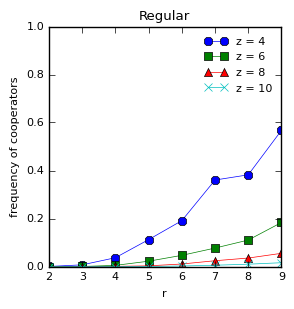
\includegraphics[width=\textwidth]{fig/fixed/regular.png}
			\caption{}
		\end{subfigure}
		\begin{subfigure}[b]{0.4\textwidth}
			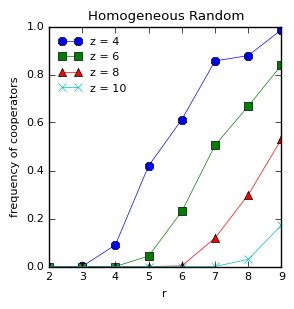
\includegraphics[width=\textwidth]{fig/fixed/homorand.png}
			\caption{}
		\end{subfigure}
		\caption{Results for Homogeneous Graphs}
		\label{fig:homographs}
	\end{figure}

	\paragraph{}As with the prisoner's dilemma, increasing the average degree $z$ makes is more difficult for cooperators to succeed.  However, the multiplicative factor $r$ does not have the same impact on cooperation in the public goods game as the temptation to defect $b$ has in the prisoner's dilemma.  While increasing $b$ makes it more difficult for cooperators to succeed in the prisoner's dilemma, increasing $r$ makes it easier for cooperators to succeed in the public goods game.
	\paragraph{}In the prisoner's dilemma case, cooperators benefit from the correlations that exist between nodes in a regular graph.  This allows the cooperators to form tight clusters that resist invasion by defectors.  However, in the case of the public good game, cooperators perform better on the random graph than on the regular graph suggesting that clustering might be disadvantageous to cooperation in the public goods game.

	\subsubsection{Heterogeneous Graphs}
    The results for three types of moderately heterogeneous small world graphs are shown in figure \ref{fig:hetergraphs}.

    \begin{figure}[h]
		\centering
		\begin{subfigure}[b]{0.4\textwidth}
			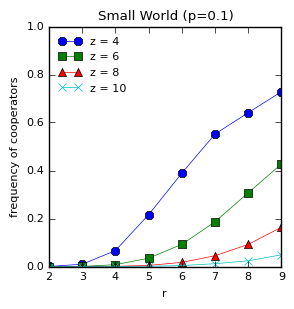
\includegraphics[width=\textwidth]{fig/fixed/sw01.png}
			\caption{}
		\end{subfigure}
		\begin{subfigure}[b]{0.4\textwidth}
			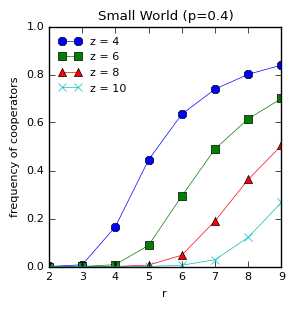
\includegraphics[width=\textwidth]{fig/fixed/sw04.png}
			\caption{}
		\end{subfigure}
		\begin{subfigure}[b]{0.4\textwidth}
			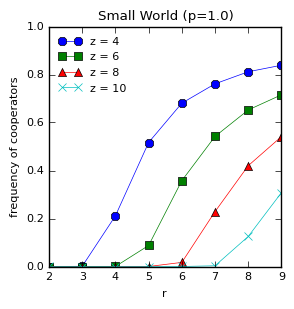
\includegraphics[width=\textwidth]{fig/fixed/heterand.png}
			\caption{}
		\end{subfigure}
		\begin{subfigure}[b]{0.4\textwidth}
			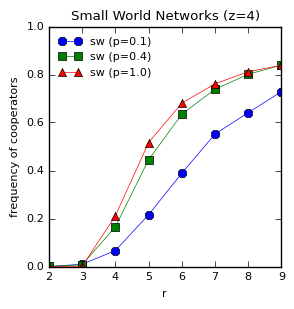
\includegraphics[width=\textwidth]{fig/fixed/smallworld.png}
			\caption{}
		\end{subfigure}
		\caption{Results for Heterogeneous Graphs}
		\label{fig:hetergraphs}
	\end{figure}

	\paragraph{}Ignoring the reversed correlation between benefit ($r$ or $b$) and level of cooperation, the results shown here are similar to the results obtained for the prisoner's dilemma.  Cooperators perform slightly better on small world networks with $p=1.0$ compared to small world networks with $p=0.4$ while their performance when $p=0.1$ is significantly worse than either of the other two cases.  As $p$ increases, the clustering coefficient decreases and heterogeneity increases.  As with the prisoner's dilemma, the results show that heterogeneity may play a more significant role in promoting cooperation than the formation of tight clusters.

	\subsubsection{Scale Free Networks}
	The results for two types of scale free graphs are shown in figure \ref{fig:sfreenets}.

	\begin{figure}[h]
		\centering
		\begin{subfigure}[b]{0.4\textwidth}
			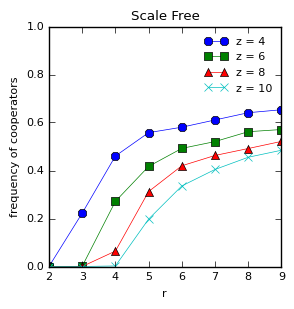
\includegraphics[width=\textwidth]{fig/fixed/sfree.png}
			\caption{}
		\end{subfigure}
		\begin{subfigure}[b]{0.4\textwidth}
			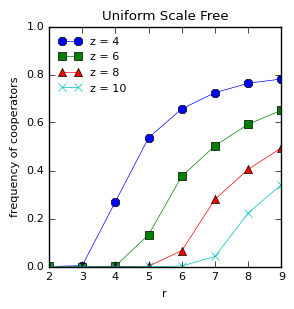
\includegraphics[width=\textwidth]{fig/fixed/usfree.png}
			\caption{}
		\end{subfigure}
		\begin{subfigure}[b]{0.4\textwidth}
			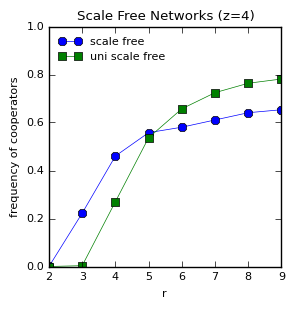
\includegraphics[width=\textwidth]{fig/fixed/scalefreeall.png}
			\caption{}
		\end{subfigure}
		\caption{Results for Scale Free Networks}
		\label{fig:sfreenets}
	\end{figure}

	\paragraph{}The results show that as average degree $z$ increases, cooperators face similar challenges to those faced by cooperators on other network types.  This is different from the result obtained for the prisoner's dilemma on scale free networks, where increasing average degree $z$ promotes cooperation.

	\paragraph{}In the prisoner's dilemma, removing age correlation from the network connections had a detrimental impact on cooperation especially for large values of the temptation to defect $b$.  However, in the public goods game, the impact of age correlation appears to be mixed.  The advantage of age correlation for small values of $r$ is significant.  However, as $r$ increases, the benefits of age correlation decrease until $r=6$ at which point cooperators perform better on a uniform scale free network.

	\subsubsection{Comparison of Network Types}
	Figure \ref{fig:compfixed} present the results in a way that allows the performance of cooperators on different graph types to be directly compared.

	\begin{figure}[h]
		\centering
		\begin{subfigure}[b]{0.4\textwidth}
			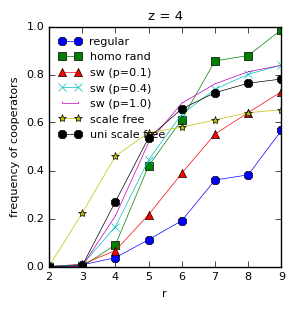
\includegraphics[width=\textwidth]{fig/fixed/z4all.png}
			\caption{}
		\end{subfigure}
		\begin{subfigure}[b]{0.4\textwidth}
			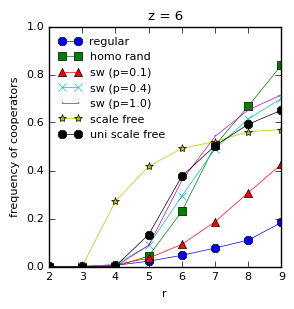
\includegraphics[width=\textwidth]{fig/fixed/z6all.png}
			\caption{}
		\end{subfigure}
		\begin{subfigure}[b]{0.4\textwidth}
			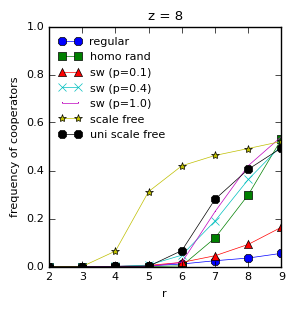
\includegraphics[width=\textwidth]{fig/fixed/z8all.png}
			\caption{}
		\end{subfigure}
		\begin{subfigure}[b]{0.4\textwidth}
			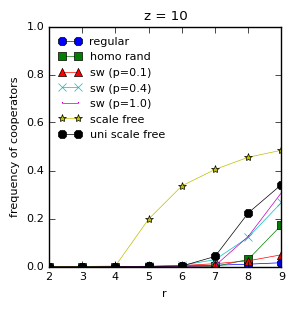
\includegraphics[width=\textwidth]{fig/fixed/z10all.png}
			\caption{}
		\end{subfigure}
		\caption{Comparison of Results for Fixed Network Types}
		\label{fig:compfixed}
	\end{figure}

	\paragraph{}It is clear that the performance of cooperators is best on scale free networks up to a critical point $r^*$.  For $r>r^*$, cooperators are able to perform better on other networks.  The benefits of increased $r$ appear to level off for cooperators on scale free networks while cooperators on other networks continue to benefit from increased $r$.  The critical point occurs at $r=5$ for $z=4$ and $r=7$ for $z=6$.  Another critical point appears to occur at $r=9$ for $z=8$ and extrapolating the curves for $z=10$ indicates that another critical point exists for some value of $r>9$.

	\subsection{Results for Dynamic Network Structure}
	As with the case of experiments performed for fixed network structure, the authors of the studies reviewed in section \ref{evo-net-topology} performed a large number of simulations in order to validate that their results were robust to fluctuations in the starting conditions.  The parameters used for those studies are shown in table \ref{table:param-values-dynamic-net-sim}.
	\paragraph{}The results presented in this paper were generated using a smaller number of generations and fewer simulations.  In the future, additional simulations can be performed to validate the robustness of the results.  A comparison of the parameters used in this study and those used in the reviewed literature is provided in table \ref{table:param-values-dynamic-net-sim}.

	\begin{table}[h!]
		\begin{center}
		\begin{tabu} to \textwidth {X[0.66,l,m]X[0.17,c,m]X[0.17,c,m]}
		\toprule
		Parameter&Value Used in Previous Studies&Value Used in This Study\\
		\midrule
		Number of agents ($N$)&$10^3$&$10^3$\\
		Number of generations per simulation&$10^8$&$10^5$\\
		Number of graph instantiations&$10$&$5$\\
		Number of simulations per graph instantiation&$10$&$5$\\
		\bottomrule
		\end{tabu}
		\caption{Parameter Values for Dynamic Network Simulations}
		\label{table:param-values-dynamic-net-sim}
		\end{center}
	\end{table}

	\paragraph{}In this study, reputation-based partner switching as described in \cite{Fu2008} was not incorporated in to the experiments.  Experiments were conducted for several different values of the average degree $z$ and the time scales ratio $W$.  In these experiments, strong selection is used with $\beta_e=\beta_a=10$ while the studies cited earlier use weak selection with $\beta_e=\beta_a=0.005$.  The following section reviews the results.
	\paragraph{} The results for of the experiments are presented in figure \ref{fig:dynamicnets}.

		\begin{figure}[h]
		\centering
		\begin{subfigure}[b]{0.4\textwidth}
			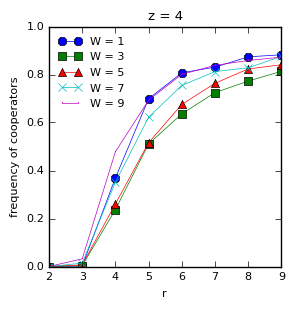
\includegraphics[width=\textwidth]{fig/dynamic/pswitch-z4.png}
			\caption{}
		\end{subfigure}
		\begin{subfigure}[b]{0.4\textwidth}
			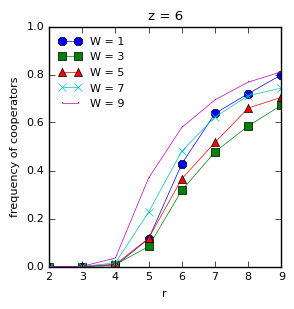
\includegraphics[width=\textwidth]{fig/dynamic/pswitch-z6.png}
			\caption{}
		\end{subfigure}
		\begin{subfigure}[b]{0.4\textwidth}
			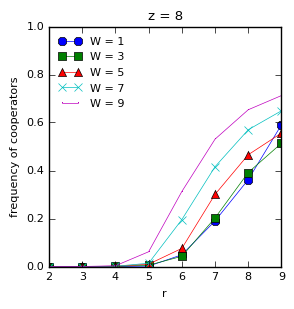
\includegraphics[width=\textwidth]{fig/dynamic/pswitch-z8.png}
			\caption{}
		\end{subfigure}
		\begin{subfigure}[b]{0.4\textwidth}
			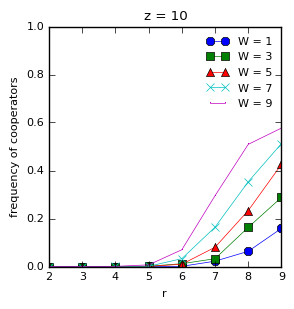
\includegraphics[width=\textwidth]{fig/dynamic/pswitch-z10.png}
			\caption{}
		\end{subfigure}
		\caption{Results for Dynamic Networks}
		\label{fig:dynamicnets}
	\end{figure}

	\paragraph{}As expected, increasing the average degree $z$ has an adverse impact on cooperation.  In general, increasing $W$ benefits cooperation.  However, for $z=4$ and $z=6$, setting $W=1$ produces results that are better than expected.
	\paragraph{}Figure \ref{fig:compdynamicfixed} compares the performance of cooperators when they inhabit a dynamic network to their performance on the three fixed networks that provided the largest boost to cooperation.  In each case, the dynamic network results presented are for $W=9$.

	\begin{figure}[h]
		\centering
		\begin{subfigure}[b]{0.4\textwidth}
			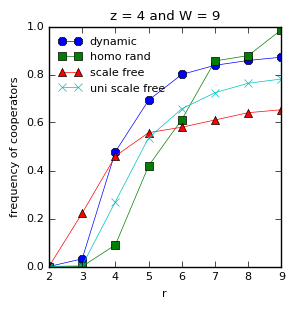
\includegraphics[width=\textwidth]{fig/dynamic/z4dynfix.png}
			\caption{}
		\end{subfigure}
		\begin{subfigure}[b]{0.4\textwidth}
			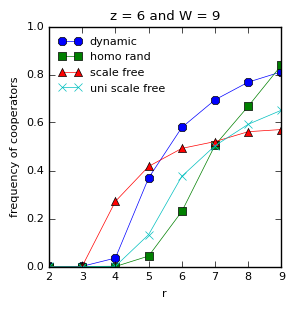
\includegraphics[width=\textwidth]{fig/dynamic/z6dynfix.png}
			\caption{}
		\end{subfigure}
		\begin{subfigure}[b]{0.4\textwidth}
			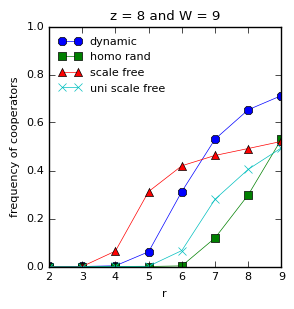
\includegraphics[width=\textwidth]{fig/dynamic/z8dynfix.png}
			\caption{}
		\end{subfigure}
		\begin{subfigure}[b]{0.4\textwidth}
			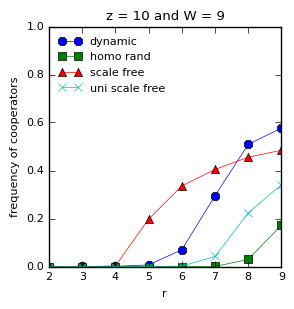
\includegraphics[width=\textwidth]{fig/dynamic/z10dynfix.png}
			\caption{}
		\end{subfigure}
		\caption{Comparison of Results for Fixed and Dynamic Networks}
		\label{fig:compdynamicfixed}
	\end{figure}

	\paragraph{}The results are mixed.  The dynamic network provides more support for cooperation when $r$ is large except for the cases when $z=4$.  However, for smaller values of $r$, the scale free network provides more benefits to cooperators.
	\paragraph{}When $z=4$, the homogeneous random network is able to provide better results than the dynamic network for $r=9$.  This is surprising since the links in the random network are created randomly while the links in the dynamic network are created following a heuristic that should result in a network that promotes cooperation.

	\section{Conclusion and Future Work}
	While there are some similarities between the impact of network topology on the emergence of cooperation in the prisoner's dilemma and public goods games, there are several differences that warrant further investigation.

	\begin{itemize}
		\item In the prisoner's dilemma, the level of cooperation is reduced as the temptation to defect $b$ increases while in the public goods game cooperation improves as the multiplier $r$ increases.
		\item In the prisoner's dilemma, cooperators fare worse on a homogeneous random graph than on a regular graph.  The reason given for this observation is that random graphs reduce the ability of cooperators to form tight clusters that can resist invasion by defectors.  In the public goods game, cooperators are able to perform significantly better on a homogeneous random graph than on a regular graph.  This begs the question how cooperators can fare so well in an environment that doesn't appear to promote the formation of tight clusters.
		\item In the prisoner's dilemma, when the game is played on a scale free network, the level of cooperation increases as the average degree increases.  This sets scale free networks apart from other network types where increasing z make it harder for cooperation to emerge.  In the public goods game, scale free networks provide no such immunity from increasing average degree.
		\item In the prisoner's dilemma, the introduction of age correlation due to preferential attachment provided a significant boost to cooperation.  In the public goods game, the impact of age correlations is mixed.
	\end{itemize}

	\paragraph{}The items listed above suggest that the promotion of cooperation in public goods games may require different features in social networks than those required by the prisoner's dilemma.  This is not surprising given the differences between the two games:

	\begin{itemize}
		\item In the prisoner's dilemma game, any increase in $b$ goes directly to defectors.  Cooperators do not benefit at all from an increase in $b$.  In the public goods game, both cooperators and defectors benefit from an increase in $r$.  Defectors receive more benefit because they do not pay a cost to participate.  However, since the cost is fixed, the percentage difference between the payouts for the two types of agents decreases as $r$ increases thus reducing the fitness advantage defectors have over cooperators.
		\item The prisoner's dilemma is played between two agents.  Therefore, an agent's performance only depends on the strategies followed by its direct neighbors.  In the public goods game, an agent's performance depends not only on its neighbor's strategy but also on its neighbor's neighbors' strategies.  Therefore, even if a cluster of friendly cooperators surrounds an agent, it can still be negatively impacted if its neighbors are not so lucky.
	\end{itemize}

	\paragraph{} A potential fruitful avenue for future research is gaining a better understanding of the features of networks that provide benefits to cooperators in the public goods game.
	\paragraph{}In this study, only a preliminary investigation into the impact of dynamic networks on public goods game was performed.  To align with other studies, future work should include conducting experiments using weak selection with smaller values for $\beta$.  In addition, the use of reputation to drive the linking process should be incorporated in order to evaluate the benefits of using reputation as a guide to selecting partners.  A social norm driven reputation mechanism like the one used in \cite{Maloney2015a} could be used to evaluate the reputations of potential partners.  Finally, a reinforcement learning approach like the one used in \cite{Macy1991} should be investigate to see if it can explain the emergence of cooperation in public goods games.

    \bibliography{../references}
    \bibliographystyle{ieeetr}
\end{document}